% The BLAKE2 data model [RFC 7693, §2.4]: message bytes form w-bit words in little-endian order
% (w = 64 for BLAKE2b, 32 for BLAKE2s), and the digest is the chain value written out in
% little-endian order.
% Original drawing for the Hash library.
\documentclass[tikz,border=6pt]{standalone}
\usepackage[T1]{fontenc}
\usepackage{lmodern}
% Shared style for the Hash diagrams.
% Palette: Okabe–Ito (colour-blind safe). Every diagram is drawn on an opaque white card so it
% stays legible on dark page themes.
\usetikzlibrary{arrows.meta,positioning,calc,fit,backgrounds}
\definecolor{hsblue}{HTML}{0072B2}
\definecolor{hsorange}{HTML}{E69F00}
\definecolor{hsgreen}{HTML}{009E73}
\definecolor{hsvermilion}{HTML}{D55E00}
\definecolor{hspurple}{HTML}{CC79A7}
\definecolor{hsink}{HTML}{1F2933}
\tikzset{
  >={Stealth[length=2.2mm]},
  every node/.style={font=\sffamily\small, text=hsink},
  wire/.style={draw=hsink, line width=0.6pt, ->},
  reg/.style={draw=hsink, line width=0.6pt, fill=hsblue!12, minimum width=9mm, minimum height=7mm},
  fn/.style={draw=hsink, line width=0.6pt, fill=hsorange!25, rounded corners=2pt, minimum width=10mm, minimum height=6mm},
  input/.style={draw=hsink, line width=0.6pt, fill=hsgreen!20, minimum width=9mm, minimum height=6mm},
  add/.style={circle, draw=hsink, line width=0.6pt, fill=white, inner sep=0pt, minimum size=5mm, font=\sffamily\bfseries},
  card/.style={fill=white, rounded corners=4pt},
}

\begin{document}
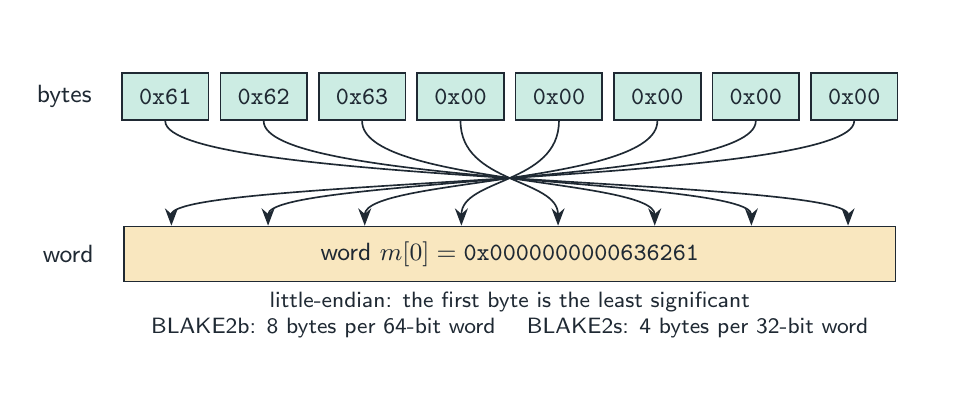
\begin{tikzpicture}
  \def\bw{1.25}
  \foreach \v [count=\i from 0] in {61,62,63,00,00,00,00,00} {
    \node[input, minimum width=11mm] (B\i) at (\i*\bw, 0) {\texttt{0x\v}};
  }
  \node[anchor=east] at ($(B0.west)+(-0.25,0)$) {bytes};
  \node[reg, minimum width=8*\bw cm - 2mm, fill=hsorange!25] (W)
    at ($(B0)!0.5!(B7)+(0,-2.0)$) {word $m[0] = \mathtt{0x0000000000636261}$};
  \node[anchor=east] at ($(W.west)+(-0.25,0)$) {word};
  \foreach \i in {0,...,7} {
    \draw[wire] (B\i.south) .. controls +(0,-0.8) and +(0,0.6)
      .. ($(W.north east)!{(\i+0.5)/8}!(W.north west)$);
  }
  \node[anchor=north, font=\sffamily\footnotesize, align=center] at (W.south)
    {little-endian: the first byte is the least significant\\
     BLAKE2b: 8 bytes per 64-bit word \quad BLAKE2s: 4 bytes per 32-bit word};
  \begin{scope}[on background layer]
    \node[card, fit=(B0)(B7)(W), inner sep=10pt, xshift=-4mm, minimum width=11.4cm,
      minimum height=4.4cm, yshift=-3mm] {};
  \end{scope}
\end{tikzpicture}
\end{document}
